% Golden fixture: legacy EECS 16A markup driven through the compatibility shim.
% Everything below the preamble is written the way the existing question bank
% writes it -- \qns, \qitem inside an enumerate, \sol, qunlist, \def\title.
\DocumentMetadata{
  lang       = en-US,
  pdfversion = 2.0,
  testphase  = {phase-III,math,table,graphic,firstaid},
}
\documentclass[sol]{latexa11y-assignment}

\usepackage{tikz}
\usepackage{latexa11y-compat-ee16}

\setcoursenumber{EECS 16A}
\setcoursename{Designing Information Devices and Systems I}
\setsemester{Spring 2026}

\begin{document}

% The legacy argument-less form: recovered by the shim at \begin{document}.
\def\title{Homework 9}

\maketitle

\begin{qunlist}

\qns{Noisy Images}

We model the measurement as a linear system.

\begin{enumerate}
\qitem
Express the image vector in terms of the measurement matrix.

\sol{Invert the measurement matrix and apply it to the observations.}

\qitem
State the condition under which that inverse exists.

\sol{The measurement matrix must be square and full rank.}
\end{enumerate}

\qns{Circuit Analysis}

\begin{Described}{A single resistor R1 connecting node A to ground.}
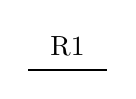
\begin{tikzpicture}
  \draw (0,0) -- (1,0);
  \node at (0.5,0.3) {R1};
\end{tikzpicture}
\end{Described}

\begin{enumerate}
\qitem
Find the current through the resistor.

\sol{Apply Ohm's law.}
\end{enumerate}

\q{10}{A Question Worth Points}

\begin{enumerate}
\qitem
Show your working.

\ans{Two amperes.}
\end{enumerate}

\end{qunlist}

\end{document}
